% Created by tikzDevice version 0.12.3.1 on 2021-09-17 14:35:45
% !TEX encoding = UTF-8 Unicode
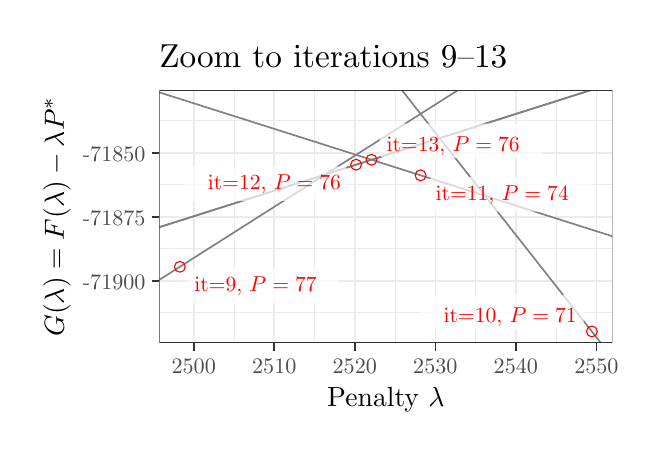
\begin{tikzpicture}[x=1pt,y=1pt]
\definecolor{fillColor}{RGB}{255,255,255}
\path[use as bounding box,fill=fillColor,fill opacity=0.00] (0,0) rectangle (216.81,144.54);
\begin{scope}
\path[clip] (  0.00,  0.00) rectangle (216.81,144.54);
\definecolor{drawColor}{RGB}{255,255,255}
\definecolor{fillColor}{RGB}{255,255,255}

\path[draw=drawColor,line width= 0.6pt,line join=round,line cap=round,fill=fillColor] (  0.00,  0.00) rectangle (216.81,144.54);
\end{scope}
\begin{scope}
\path[clip] ( 47.55, 30.61) rectangle (211.31,121.94);
\definecolor{fillColor}{RGB}{255,255,255}

\path[fill=fillColor] ( 47.55, 30.61) rectangle (211.31,121.94);
\definecolor{drawColor}{gray}{0.92}

\path[draw=drawColor,line width= 0.3pt,line join=round] ( 47.55, 41.54) --
	(211.31, 41.54);

\path[draw=drawColor,line width= 0.3pt,line join=round] ( 47.55, 64.64) --
	(211.31, 64.64);

\path[draw=drawColor,line width= 0.3pt,line join=round] ( 47.55, 87.75) --
	(211.31, 87.75);

\path[draw=drawColor,line width= 0.3pt,line join=round] ( 47.55,110.85) --
	(211.31,110.85);

\path[draw=drawColor,line width= 0.3pt,line join=round] ( 74.55, 30.61) --
	( 74.55,121.94);

\path[draw=drawColor,line width= 0.3pt,line join=round] (103.66, 30.61) --
	(103.66,121.94);

\path[draw=drawColor,line width= 0.3pt,line join=round] (132.76, 30.61) --
	(132.76,121.94);

\path[draw=drawColor,line width= 0.3pt,line join=round] (161.86, 30.61) --
	(161.86,121.94);

\path[draw=drawColor,line width= 0.3pt,line join=round] (190.96, 30.61) --
	(190.96,121.94);

\path[draw=drawColor,line width= 0.6pt,line join=round] ( 47.55, 53.09) --
	(211.31, 53.09);

\path[draw=drawColor,line width= 0.6pt,line join=round] ( 47.55, 76.19) --
	(211.31, 76.19);

\path[draw=drawColor,line width= 0.6pt,line join=round] ( 47.55, 99.30) --
	(211.31, 99.30);

\path[draw=drawColor,line width= 0.6pt,line join=round] ( 60.00, 30.61) --
	( 60.00,121.94);

\path[draw=drawColor,line width= 0.6pt,line join=round] ( 89.11, 30.61) --
	( 89.11,121.94);

\path[draw=drawColor,line width= 0.6pt,line join=round] (118.21, 30.61) --
	(118.21,121.94);

\path[draw=drawColor,line width= 0.6pt,line join=round] (147.31, 30.61) --
	(147.31,121.94);

\path[draw=drawColor,line width= 0.6pt,line join=round] (176.41, 30.61) --
	(176.41,121.94);

\path[draw=drawColor,line width= 0.6pt,line join=round] (205.51, 30.61) --
	(205.51,121.94);
\definecolor{drawColor}{gray}{0.50}

\path[draw=drawColor,line width= 0.6pt,line join=round] (-116.21,-50.61) -- (375.07,261.44);

\path[draw=drawColor,line width= 0.6pt,line join=round] (-116.21,441.37) -- (375.07,-182.73);

\path[draw=drawColor,line width= 0.6pt,line join=round] (-116.21,173.18) -- (375.07, 17.15);

\path[draw=drawColor,line width= 0.6pt,line join=round] (-116.21, 20.43) -- (375.07,176.46);

\path[draw=drawColor,line width= 0.6pt,line join=round] (-116.21, 20.43) -- (375.07,176.46);
\definecolor{fillColor}{RGB}{255,255,255}

\path[fill=fillColor,fill opacity=0.70] ( 59.72, 45.04) --
	(110.42, 45.04) --
	(110.34, 45.04) --
	(110.66, 45.05) --
	(110.98, 45.11) --
	(111.27, 45.23) --
	(111.55, 45.39) --
	(111.80, 45.59) --
	(112.01, 45.83) --
	(112.18, 46.10) --
	(112.31, 46.39) --
	(112.38, 46.70) --
	(112.41, 47.02) --
	(112.41, 47.02) --
	(112.41, 55.52) --
	(112.41, 55.52) --
	(112.38, 55.84) --
	(112.31, 56.15) --
	(112.18, 56.45) --
	(112.01, 56.72) --
	(111.80, 56.96) --
	(111.55, 57.16) --
	(111.27, 57.32) --
	(110.98, 57.43) --
	(110.66, 57.50) --
	(110.42, 57.51) --
	( 59.72, 57.51) --
	( 59.96, 57.50) --
	( 59.64, 57.51) --
	( 59.32, 57.47) --
	( 59.01, 57.38) --
	( 58.72, 57.25) --
	( 58.46, 57.06) --
	( 58.23, 56.84) --
	( 58.04, 56.59) --
	( 57.89, 56.30) --
	( 57.79, 56.00) --
	( 57.73, 55.68) --
	( 57.73, 55.52) --
	( 57.73, 47.02) --
	( 57.73, 47.18) --
	( 57.73, 46.86) --
	( 57.79, 46.55) --
	( 57.89, 46.24) --
	( 58.04, 45.96) --
	( 58.23, 45.70) --
	( 58.46, 45.48) --
	( 58.72, 45.30) --
	( 59.01, 45.16) --
	( 59.32, 45.08) --
	( 59.64, 45.04) --
	cycle;
\end{scope}
\begin{scope}
\path[clip] ( 47.55, 30.61) rectangle (211.31,121.94);
\definecolor{drawColor}{RGB}{255,0,0}

\node[text=drawColor,anchor=base west,inner sep=0pt, outer sep=0pt, scale=  0.78] at ( 60.22, 49.16) {it=9, $P=77$};
\definecolor{fillColor}{RGB}{255,255,255}

\path[fill=fillColor,fill opacity=0.70] (144.00, 35.38) --
	(198.93, 35.38) --
	(198.85, 35.38) --
	(199.17, 35.40) --
	(199.49, 35.46) --
	(199.79, 35.57) --
	(200.06, 35.73) --
	(200.31, 35.94) --
	(200.52, 36.17) --
	(200.69, 36.45) --
	(200.82, 36.74) --
	(200.90, 37.05) --
	(200.92, 37.37) --
	(200.92, 37.37) --
	(200.92, 45.87) --
	(200.92, 45.87) --
	(200.90, 46.19) --
	(200.82, 46.50) --
	(200.69, 46.79) --
	(200.52, 47.06) --
	(200.31, 47.30) --
	(200.06, 47.51) --
	(199.79, 47.67) --
	(199.49, 47.78) --
	(199.17, 47.84) --
	(198.93, 47.86) --
	(144.00, 47.86) --
	(144.24, 47.84) --
	(143.92, 47.86) --
	(143.60, 47.82) --
	(143.30, 47.73) --
	(143.01, 47.59) --
	(142.75, 47.41) --
	(142.51, 47.19) --
	(142.32, 46.93) --
	(142.17, 46.65) --
	(142.07, 46.35) --
	(142.02, 46.03) --
	(142.02, 45.87) --
	(142.02, 37.37) --
	(142.02, 37.53) --
	(142.02, 37.21) --
	(142.07, 36.89) --
	(142.17, 36.59) --
	(142.32, 36.31) --
	(142.51, 36.05) --
	(142.75, 35.83) --
	(143.01, 35.65) --
	(143.30, 35.51) --
	(143.60, 35.42) --
	(143.92, 35.38) --
	cycle;
\end{scope}
\begin{scope}
\path[clip] ( 47.55, 30.61) rectangle (211.31,121.94);
\definecolor{drawColor}{RGB}{255,0,0}

\node[text=drawColor,anchor=base east,inner sep=0pt, outer sep=0pt, scale=  0.78] at (198.42, 37.88) {it=10, $P=71$};
\definecolor{fillColor}{RGB}{255,255,255}

\path[fill=fillColor,fill opacity=0.70] (146.91, 78.08) --
	(201.84, 78.08) --
	(201.76, 78.08) --
	(202.08, 78.10) --
	(202.39, 78.16) --
	(202.69, 78.27) --
	(202.97, 78.43) --
	(203.21, 78.63) --
	(203.43, 78.87) --
	(203.60, 79.14) --
	(203.72, 79.44) --
	(203.80, 79.75) --
	(203.82, 80.07) --
	(203.82, 80.07) --
	(203.82, 88.57) --
	(203.82, 88.57) --
	(203.80, 88.89) --
	(203.72, 89.20) --
	(203.60, 89.49) --
	(203.43, 89.76) --
	(203.21, 90.00) --
	(202.97, 90.21) --
	(202.69, 90.37) --
	(202.39, 90.48) --
	(202.08, 90.54) --
	(201.84, 90.56) --
	(146.91, 90.56) --
	(147.15, 90.54) --
	(146.83, 90.56) --
	(146.51, 90.52) --
	(146.20, 90.43) --
	(145.91, 90.29) --
	(145.65, 90.11) --
	(145.42, 89.89) --
	(145.23, 89.63) --
	(145.08, 89.35) --
	(144.98, 89.05) --
	(144.93, 88.73) --
	(144.92, 88.57) --
	(144.92, 80.07) --
	(144.93, 80.23) --
	(144.93, 79.91) --
	(144.98, 79.59) --
	(145.08, 79.29) --
	(145.23, 79.01) --
	(145.42, 78.75) --
	(145.65, 78.53) --
	(145.91, 78.35) --
	(146.20, 78.21) --
	(146.51, 78.12) --
	(146.83, 78.08) --
	cycle;
\end{scope}
\begin{scope}
\path[clip] ( 47.55, 30.61) rectangle (211.31,121.94);
\definecolor{drawColor}{RGB}{255,0,0}

\node[text=drawColor,anchor=base west,inner sep=0pt, outer sep=0pt, scale=  0.78] at (147.42, 82.21) {it=11, $P=74$};
\definecolor{fillColor}{RGB}{255,255,255}

\path[fill=fillColor,fill opacity=0.70] ( 58.81, 81.93) --
	(113.74, 81.93) --
	(113.66, 81.93) --
	(113.98, 81.94) --
	(114.29, 82.01) --
	(114.59, 82.12) --
	(114.87, 82.28) --
	(115.12, 82.48) --
	(115.33, 82.72) --
	(115.50, 82.99) --
	(115.62, 83.29) --
	(115.70, 83.60) --
	(115.73, 83.92) --
	(115.73, 83.92) --
	(115.73, 92.42) --
	(115.73, 92.42) --
	(115.70, 92.74) --
	(115.62, 93.05) --
	(115.50, 93.34) --
	(115.33, 93.61) --
	(115.12, 93.85) --
	(114.87, 94.05) --
	(114.59, 94.21) --
	(114.29, 94.33) --
	(113.98, 94.39) --
	(113.74, 94.41) --
	( 58.81, 94.41) --
	( 59.05, 94.39) --
	( 58.73, 94.40) --
	( 58.41, 94.37) --
	( 58.10, 94.28) --
	( 57.81, 94.14) --
	( 57.55, 93.96) --
	( 57.32, 93.74) --
	( 57.13, 93.48) --
	( 56.98, 93.20) --
	( 56.88, 92.89) --
	( 56.83, 92.58) --
	( 56.82, 92.42) --
	( 56.82, 83.92) --
	( 56.83, 84.08) --
	( 56.83, 83.76) --
	( 56.88, 83.44) --
	( 56.98, 83.14) --
	( 57.13, 82.85) --
	( 57.32, 82.60) --
	( 57.55, 82.38) --
	( 57.81, 82.20) --
	( 58.10, 82.06) --
	( 58.41, 81.97) --
	( 58.73, 81.93) --
	cycle;
\end{scope}
\begin{scope}
\path[clip] ( 47.55, 30.61) rectangle (211.31,121.94);
\definecolor{drawColor}{RGB}{255,0,0}

\node[text=drawColor,anchor=base east,inner sep=0pt, outer sep=0pt, scale=  0.78] at (113.23, 86.06) {it=12, $P=76$};
\definecolor{fillColor}{RGB}{255,255,255}

\path[fill=fillColor,fill opacity=0.70] (129.20, 97.43) --
	(184.13, 97.43) --
	(184.05, 97.43) --
	(184.37, 97.44) --
	(184.68, 97.51) --
	(184.98, 97.62) --
	(185.26, 97.78) --
	(185.50, 97.98) --
	(185.72, 98.22) --
	(185.89, 98.49) --
	(186.01, 98.79) --
	(186.09, 99.10) --
	(186.11, 99.42) --
	(186.11, 99.42) --
	(186.11,107.92) --
	(186.11,107.92) --
	(186.09,108.24) --
	(186.01,108.55) --
	(185.89,108.84) --
	(185.72,109.11) --
	(185.50,109.35) --
	(185.26,109.56) --
	(184.98,109.72) --
	(184.68,109.83) --
	(184.37,109.89) --
	(184.13,109.91) --
	(129.20,109.91) --
	(129.44,109.89) --
	(129.12,109.91) --
	(128.80,109.87) --
	(128.49,109.78) --
	(128.20,109.64) --
	(127.94,109.46) --
	(127.71,109.24) --
	(127.52,108.98) --
	(127.37,108.70) --
	(127.27,108.40) --
	(127.21,108.08) --
	(127.21,107.92) --
	(127.21, 99.42) --
	(127.21, 99.58) --
	(127.21, 99.26) --
	(127.27, 98.94) --
	(127.37, 98.64) --
	(127.52, 98.36) --
	(127.71, 98.10) --
	(127.94, 97.88) --
	(128.20, 97.70) --
	(128.49, 97.56) --
	(128.80, 97.47) --
	(129.12, 97.43) --
	cycle;
\end{scope}
\begin{scope}
\path[clip] ( 47.55, 30.61) rectangle (211.31,121.94);
\definecolor{drawColor}{RGB}{255,0,0}

\node[text=drawColor,anchor=base west,inner sep=0pt, outer sep=0pt, scale=  0.78] at (129.70, 99.93) {it=13, $P=76$};

\path[draw=drawColor,line width= 0.4pt,line join=round,line cap=round] ( 54.99, 58.14) circle (  1.96);

\path[draw=drawColor,line width= 0.4pt,line join=round,line cap=round] (203.87, 34.76) circle (  1.96);

\path[draw=drawColor,line width= 0.4pt,line join=round,line cap=round] (141.97, 91.18) circle (  1.96);

\path[draw=drawColor,line width= 0.4pt,line join=round,line cap=round] (118.67, 95.03) circle (  1.96);

\path[draw=drawColor,line width= 0.4pt,line join=round,line cap=round] (124.26, 96.81) circle (  1.96);
\definecolor{drawColor}{gray}{0.20}

\path[draw=drawColor,line width= 0.6pt,line join=round,line cap=round] ( 47.55, 30.61) rectangle (211.31,121.94);
\end{scope}
\begin{scope}
\path[clip] (  0.00,  0.00) rectangle (216.81,144.54);
\definecolor{drawColor}{gray}{0.30}

\node[text=drawColor,anchor=base east,inner sep=0pt, outer sep=0pt, scale=  0.80] at ( 42.60, 50.07) {-71900};

\node[text=drawColor,anchor=base east,inner sep=0pt, outer sep=0pt, scale=  0.80] at ( 42.60, 73.18) {-71875};

\node[text=drawColor,anchor=base east,inner sep=0pt, outer sep=0pt, scale=  0.80] at ( 42.60, 96.28) {-71850};
\end{scope}
\begin{scope}
\path[clip] (  0.00,  0.00) rectangle (216.81,144.54);
\definecolor{drawColor}{gray}{0.20}

\path[draw=drawColor,line width= 0.6pt,line join=round] ( 44.80, 53.09) --
	( 47.55, 53.09);

\path[draw=drawColor,line width= 0.6pt,line join=round] ( 44.80, 76.19) --
	( 47.55, 76.19);

\path[draw=drawColor,line width= 0.6pt,line join=round] ( 44.80, 99.30) --
	( 47.55, 99.30);
\end{scope}
\begin{scope}
\path[clip] (  0.00,  0.00) rectangle (216.81,144.54);
\definecolor{drawColor}{gray}{0.20}

\path[draw=drawColor,line width= 0.6pt,line join=round] ( 60.00, 27.86) --
	( 60.00, 30.61);

\path[draw=drawColor,line width= 0.6pt,line join=round] ( 89.11, 27.86) --
	( 89.11, 30.61);

\path[draw=drawColor,line width= 0.6pt,line join=round] (118.21, 27.86) --
	(118.21, 30.61);

\path[draw=drawColor,line width= 0.6pt,line join=round] (147.31, 27.86) --
	(147.31, 30.61);

\path[draw=drawColor,line width= 0.6pt,line join=round] (176.41, 27.86) --
	(176.41, 30.61);

\path[draw=drawColor,line width= 0.6pt,line join=round] (205.51, 27.86) --
	(205.51, 30.61);
\end{scope}
\begin{scope}
\path[clip] (  0.00,  0.00) rectangle (216.81,144.54);
\definecolor{drawColor}{gray}{0.30}

\node[text=drawColor,anchor=base,inner sep=0pt, outer sep=0pt, scale=  0.80] at ( 60.00, 19.62) {2500};

\node[text=drawColor,anchor=base,inner sep=0pt, outer sep=0pt, scale=  0.80] at ( 89.11, 19.62) {2510};

\node[text=drawColor,anchor=base,inner sep=0pt, outer sep=0pt, scale=  0.80] at (118.21, 19.62) {2520};

\node[text=drawColor,anchor=base,inner sep=0pt, outer sep=0pt, scale=  0.80] at (147.31, 19.62) {2530};

\node[text=drawColor,anchor=base,inner sep=0pt, outer sep=0pt, scale=  0.80] at (176.41, 19.62) {2540};

\node[text=drawColor,anchor=base,inner sep=0pt, outer sep=0pt, scale=  0.80] at (205.51, 19.62) {2550};
\end{scope}
\begin{scope}
\path[clip] (  0.00,  0.00) rectangle (216.81,144.54);
\definecolor{drawColor}{RGB}{0,0,0}

\node[text=drawColor,anchor=base,inner sep=0pt, outer sep=0pt, scale=  1.00] at (129.43,  7.63) {Penalty $\lambda$};
\end{scope}
\begin{scope}
\path[clip] (  0.00,  0.00) rectangle (216.81,144.54);
\definecolor{drawColor}{RGB}{0,0,0}

\node[text=drawColor,rotate= 90.00,anchor=base,inner sep=0pt, outer sep=0pt, scale=  1.00] at ( 13.04, 76.27) {$G(\lambda)=F(\lambda)-\lambda P^*$};
\end{scope}
\begin{scope}
\path[clip] (  0.00,  0.00) rectangle (216.81,144.54);
\definecolor{drawColor}{RGB}{0,0,0}

\node[text=drawColor,anchor=base west,inner sep=0pt, outer sep=0pt, scale=  1.20] at ( 47.55,129.99) {Zoom to iterations 9--13};
\end{scope}
\end{tikzpicture}
